\documentclass[conference]{IEEEtran}
\IEEEoverridecommandlockouts
% The preceding line is only needed to identify funding in the first footnote. If that is unneeded, please comment it out.
\usepackage{cite}
\usepackage{amsmath,amssymb,amsfonts}
\usepackage{algorithmic}
\usepackage{graphicx}
\usepackage{textcomp}
\usepackage{xcolor}
\usepackage{booktabs}
\usepackage{multirow}
\usepackage{url}
\usepackage{hyperref}

\hypersetup{
    colorlinks=false,
    hidelinks,
}

\def\BibTeX{{\rm B\kern-.05em{\sc i\kern-.025em b}\kern-.08em
    T\kern-.1667em\lower.7ex\hbox{E}\kern-.125emX}}

\begin{document}

\title{Robustness of Roman Urdu Sentiment Classification to Orthographic Spelling Variation: A Comparative Study of Full Fine-Tuning and Parameter-Efficient Adaptation of Multilingual Transformers}

\author{\IEEEauthorblockN{Danyal Ahmed Malik}
\IEEEauthorblockA{\textit{Department of Data Science — Graduate Studies} \\
\textit{National University of Computer \& Emerging Sciences (FAST-NUCES)}\\
Islamabad, Pakistan \\
Email: i268030@isb.nu.edu.pk}
}

\maketitle

\begin{abstract}
Roman Urdu---Urdu written in Latin script---is the dominant medium for informal digital communication across South Asia, yet it lacks standardized orthography. While multilingual transformers such as mBERT and XLM-RoBERTa achieve strong results on clean benchmarks, their robustness under systematic orthographic noise remains unexamined. We present a controlled empirical study investigating whether Parameter-Efficient Fine-Tuning via Low-Rank Adaptation (LoRA) confers superior resilience compared to full fine-tuning. After auditing the 28,090-review RUWV-NSR dataset---resolving label corruption and removing 4,632 duplicates (16.49\%)---we construct graded perturbation conditions using a 10,869-pair authentic spelling-variation lexicon. We evaluate TF-IDF + Logistic Regression, mBERT, XLM-RoBERTa (full fine-tuning), and XLM-RoBERTa (LoRA) across canonical noise tiers and a $3 \times 3$ factorial grid. LoRA adaptation exhibits substantially superior resilience, incurring only 4.68\% relative Macro-F1 degradation under severe noise versus 7.01\% for full fine-tuning and 16.42\% for the classical baseline. Lexicon-driven normalization recovers 84--94\% of spelling-induced loss, whereas generic preprocessing yields zero recovery. Findings generalize across 3,000 independent e-commerce reviews.
\end{abstract}

\begin{IEEEkeywords}
Roman Urdu, Sentiment Analysis, Orthographic Robustness, Multilingual Transformers, Low-Rank Adaptation (LoRA), Parameter-Efficient Fine-Tuning (PEFT), Spelling Perturbation.
\end{IEEEkeywords}

\section{Introduction}
\label{sec:introduction}

Roman Urdu---the phonological transcription of the Urdu language using the standard 26-letter Latin alphabet---has emerged as the de facto written medium for informal digital communication across Pakistan and the broader South Asian diaspora. It permeates user reviews on e-commerce platforms, customer feedback on social media channels, and mobile instant messaging. Despite its ubiquity, Roman Urdu is strictly an unstandardized vernacular. While classical Nastaliq Urdu employs an alphabet of 36 distinct characters with formal orthographic rules, Roman Urdu lacks any centralized standardizing authority or agreed-upon phonetic mapping. Consequently, native speakers write purely by acoustic approximation. 

A single lexical item or sentiment-bearing predicate can easily manifest in several divergent spelling variations depending entirely on individual typists, regional phonology, and texting conventions. For instance, the core affirmation \textit{accha} (``good'') frequently appears as \textit{acha}, \textit{achha}, \textit{achaah}, or \textit{achaaa}; similarly, the negation \textit{nahi} (``not'') is written interchangeably as \textit{nhn}, \textit{nahin}, \textit{nhi}, or \textit{nahe}. In the context of automated Natural Language Processing (NLP), and Sentiment Analysis (SA) in particular, this extreme orthographic entropy poses a formidable challenge.

In contemporary NLP research, Pre-trained Multilingual Language Models (PMLMs) such as multilingual BERT (\mbox{mBERT})~\cite{devlin2019bert} and XLM-RoBERTa (\mbox{XLM-R})~\cite{conneau2020unsupervised} have demonstrated state-of-the-art classification performance on code-mixed and low-resource benchmarks. However, the standard evaluation paradigm in the literature remains fundamentally flawed: models are trained and tested on single, static, identically distributed (i.i.d.) random splits of a scraped corpus. When an automated classifier achieves high benchmark accuracy under such conditions, it often reflects memorization of canonical spelling forms within a closed vocabulary rather than generalized sentiment comprehension. In live production environments, incoming text exhibits uncontrolled spelling shifts that induce severe out-of-vocabulary (OOV) rates, token fragmentation, and downstream classification failure.

Recent literature explicitly acknowledges this bottleneck. Notably, Nazir et al.~\cite{nazir2025leveraging} benchmarked mBERT on code-mixed Roman Urdu and Roman Punjabi social media reviews, demonstrating strong in-domain accuracy (79.94\%) but observing that generic text preprocessing (e.g., stop-word and punctuation removal) produced only marginal improvements (2.71\%). The authors highlighted that imperfect Romanized text normalization remains an unaddressed limitation. In parallel, Khan et al.~\cite{khan2026romeva} investigated vocabulary expansion on the Roman Urdu Word Variations and Normalized Sentiment Review (RUWV-NSR) dataset~\cite{ahmed2024ruwvnsr}, focusing on embedding-space drift. However, no prior work has systematically quantified the degradation curves of multilingual transformers under controlled, graded orthographic noise for Roman Urdu, nor investigated whether adaptation strategy influences robustness.

This study directly bridges this empirical gap. Treating Roman Urdu sentiment classification as a rigorous, end-to-end data-science pipeline, we investigate the following core research questions:
\begin{enumerate}
    \item[\textbf{RQ1:}] \textit{Degradation Under Orthographic Noise:} How does sentiment classification performance degrade across increasing severity levels of authentic spelling variation for classical versus transformer-based architectures?
    \item[\textbf{RQ2:}] \textit{Parameter-Efficient vs. Full Adaptation:} Does Low-Rank Adaptation (LoRA)~\cite{hu2022lora} confer greater robustness against orthographic perturbation compared to unconstrained full fine-tuning?
    \item[\textbf{RQ3:}] \textit{Token Fragmentation Profiling:} To what extent do distinct subword tokenization schemes (WordPiece vs. SentencePiece/BPE) fragment authentic lexical variants, and how does this correlate with performance drop?
    \item[\textbf{RQ4:}] \textit{Factorial Disentanglement:} Is performance degradation predominantly driven by word substitution rate, character edit distance, or their mutual interaction?
    \item[\textbf{RQ5:}] \textit{Mitigation and Normalization:} Can lexicon-driven orthographic normalization or noise-augmented training reverse perturbation losses where generic preprocessing fails?
\end{enumerate}

To answer these questions, we perform an independent data audit on the RUWV-NSR corpus, resolving pervasive label corruption and eliminating 4,632 exact duplicate reviews (16.49\%) to establish a strictly leakage-free benchmark. Leveraging a paired lexicon of 5,244 words (10,869 authentic variant pairs), we develop a perturbation engine that constructs canonical noise tiers alongside a full $3 \times 3$ factorial grid. We benchmark four primary modeling paradigms: TF-IDF + Logistic Regression, fully fine-tuned mBERT, fully fine-tuned XLM-RoBERTa, and LoRA-adapted XLM-RoBERTa. Finally, we execute normalization ablations and validate cross-domain generalizability on 3,000 independent reviews from the Daraz.pk RUECD corpus~\cite{chandio2022sentiment}.

\section{Related Work}
\label{sec:related_work}

The literature intersecting this research encompasses two dominant trajectories: multiclass sentiment classification in code-mixed and Romanized low-resource languages, and transformer robustness under adversarial or natural orthographic perturbation.

\subsection{Multiclass Sentiment Classification in Roman Urdu}
Early computational investigations in Roman Urdu sentiment analysis relied heavily on surface-level feature engineering, employing Bag-of-Words (BoW) representations, character n-grams, and classical machine learning estimators such as Support Vector Machines (SVM), Naive Bayes, and Random Forests~\cite{chandio2022sentiment}. While character n-grams partially alleviate minor typing slips by capturing sub-word substrings, classical estimators are fundamentally incapable of modeling long-range syntactic dependencies, negation scope, and polysemy.

The introduction of multilingual pre-trained encoders catalyzed significant progress. Devlin et al.~\cite{devlin2019bert} established the efficacy of multilingual BERT (mBERT), pre-trained across 104 languages on Wikipedia corpora. Conneau et al.~\cite{conneau2020unsupervised} subsequently introduced XLM-RoBERTa (XLM-R), trained on 2.5TB of filtered CommonCrawl data in 100 languages, demonstrating substantial performance advantages in cross-lingual transfer benchmarks. 

In a notable recent study, Nazir et al.~\cite{nazir2025leveraging} proposed CMSA-mBERT for three-class sentiment analysis across 48,324 Roman Urdu and Roman Punjabi code-mixed reviews. Their model achieved a benchmark accuracy of 79.94\%, outperforming traditional ML and recurrent architectures (LSTM, BiLSTM, GRU). Crucially, the authors observed that standard preprocessing techniques (stripping stopwords, punctuation, and emojis) produced only an insubstantial 2.71\% improvement, citing unstandardized Romanized orthography as an intractable limitation. However, their experimental design was restricted to a single clean 80/20 train/test split, leaving the models' resilience to spelling noise untested.

\subsection{Vocabulary Adaptation and Embedding Stability}
Multilingual language models typically suffer from representation degradation when applied to languages absent from their pre-training corpora. Because Roman Urdu is underrepresented in mBERT and XLM-RoBERTa, native words are fragmented into highly localized subword units. 

Addressing this phenomenon, Khan et al.~\cite{khan2026romeva} introduced ROMEVA, an anchor-loss vocabulary expansion technique designed to preserve embedding-space geometry when adapting mBERT to Roman Urdu using the RUWV-NSR dataset~\cite{ahmed2024ruwvnsr}. Their findings indicated that while unconstrained naive fine-tuning disrupted the pre-trained semantic geometry more severely than constrained methods, it paradoxically achieved superior downstream classification accuracy. Nevertheless, Khan et al. focused exclusively on embedding drift rather than input-level orthographic perturbation, did not evaluate parameter-efficient tuning paradigms, and evaluated solely on unaltered review splits.

\subsection{Robustness and Perturbation Evaluation}
Assessing the brittle nature of deep neural language models under input perturbations is an active subfield. Moradi and Samwald~\cite{moradi2021evaluating} systematically evaluated transformer architectures under synthetic character-level noises (random character insertion, deletion, and swap), finding severe degradation across standard benchmarks.

However, existing perturbation benchmarks predominantly introduce synthetic typographic noise (e.g., keyboard layout typos) rather than authentic, sociolinguistically validated spelling variations. In Roman Urdu, spelling variation is not random noise but a structured phonological phenomenon. By leveraging an authentic, human-documented variation lexicon, our work provides the first controlled robustness benchmark for Roman Urdu sentiment classification.

\subsection{Parameter-Efficient Fine-Tuning (PEFT)}
As language models have scaled, parameter-efficient adaptation methods have emerged as powerful alternatives to full fine-tuning. Hu et al.~\cite{hu2022lora} introduced Low-Rank Adaptation (LoRA), which freezes the pre-trained backbone weights $W_0 \in \mathbb{R}^{d \times k}$ and injects trainable rank-decomposition matrices $\Delta W = B \cdot A$, where $B \in \mathbb{R}^{d \times r}$, $A \in \mathbb{R}^{r \times k}$, and rank $r \ll \min(d, k)$. Beyond drastically reducing trainable parameters and GPU memory overhead, recent theoretical insights suggest that constraining updates to low-rank subspaces acts as implicit regularization, mitigating catastrophic forgetting of pre-trained linguistic priors. In this paper, we hypothesize that this regularization makes LoRA inherently more resilient to input orthographic shifts than full parameter updates.

\section{Data Pipeline and Orthographic Perturbation}
\label{sec:data_pipeline}

\subsection{Data Audit, Inconsistency Resolution, and Deduplication}
Our primary experimental benchmark is constructed from the Roman Urdu Word Variations and Normalized Sentiment Review Dataset (RUWV-NSR)~\cite{ahmed2024ruwvnsr}, acquired from Mendeley Data under a CC BY 4.0 license. The corpus comprises 28,090 reviews collected across seven online domains alongside a dedicated Roman Urdu spelling-variation lexicon containing 5,244 headwords.

Prior to modeling, we performed an independent data audit that revealed critical anomalies necessitating rigorous data engineering:
\begin{enumerate}
    \item \textbf{Label Inconsistency and Typos:} Target annotations were distributed across eight conflicting string representations due to casing disparities and lexical errors (e.g., \texttt{"Neative"}). We canonicalized these into five balanced classes: \textit{very positive} ($N=5,008$), \textit{positive} ($N=6,288$), \textit{neutral} ($N=6,445$), \textit{negative} ($N=6,036$), and \textit{very negative} ($N=4,313$).
    \item \textbf{Severe Duplication and Label Contradiction:} We detected 4,632 exact duplicate reviews (16.49\% of the raw corpus). Crucially, a subset of identical textual reviews was annotated with conflicting sentiment labels across different collection runs. Retaining duplicated instances introduces direct data leakage across train/test splits and artificially inflates cross-validation metrics. Eliminating duplicates reduced the corpus to 23,458 pristine, unique reviews.
\end{enumerate}

\subsection{Lexicon Processing and Inversion}
The RUWV-NSR lexicon documents 5,219 unique headwords paired with up to five attested spelling variations. To enable rapid, deterministic perturbation and normalization, we inverted the lexicon structure into a lookup hash table mapping each authentic variant $v$ back to its canonical form $c$, computing its normalized Levenshtein edit distance as:
\begin{equation}
    d_{\text{norm}}(c, v) = \frac{\text{Levenshtein}(c, v)}{\max(|c|, |v|)}
\end{equation}
This yielded 10,869 authentic lexical variant pairs with an average Levenshtein distance of 1.76 characters.

\subsection{Leakage-Free Stratified Partitioning}
To prevent distributional bias, the deduplicated dataset ($N=23,458$) was partitioned using stratified sampling (random seed 42) into:
\begin{itemize}
    \item \textbf{Training Set (70\%):} 16,420 reviews
    \item \textbf{Validation Set (15\%):} 3,519 reviews
    \item \textbf{Test Set (15\%):} 3,519 reviews
\end{itemize}
The class distribution was precisely preserved across all splits: Neutral ($\approx 25.9\%$), Positive ($\approx 25.2\%$), Negative ($\approx 24.4\%$), Very Positive ($\approx 13.5\%$), and Very Negative ($\approx 11.0\%$).

\subsection{Controlled Perturbation Engine}
To evaluate model degradation without label drift, we engineered an authentic variant substitution engine operating strictly on the test partition ($N=3,519$). Sentences are tokenized, and each token matching a canonical headword $c \in \mathcal{L}$ is eligible for substitution with probability $p_{\text{sub}}$. When selected, the token is substituted with an authentic variant $v \in \mathcal{V}(c)$ selected according to edit-distance criteria:
\begin{enumerate}
    \item \textbf{Canonical Severity Conditions:} Four standardized tiers were operationalized: \textit{Clean} ($p_{\text{sub}} = 0\%$), \textit{Mild} ($p_{\text{sub}} = 20\%$), \textit{Moderate} ($p_{\text{sub}} = 50\%$), and \textit{Severe} ($p_{\text{sub}} = 85\%$). Across the 3,519 test instances, the average realized substitution rates were 0.0\%, 28.4\%, 50.4\%, and 80.0\% respectively, with the number of modified words per review rising monotonically from 0.00 (Clean) to 1.72 (Mild), 3.42 (Moderate), and 6.13 (Severe).
    \item \textbf{$3 \times 3$ Factorial Grid Design:} To disentangle word substitution density from character edit distance, we constructed a $3 \times 3$ factorial grid crossing word substitution density $p_{\text{sub}} \in \{25\%, 50\%, 90\%\}$ with variant selection policies: \textit{Low Distance} ($\min_{v} d(c,v)$), \textit{Random Distance} (uniform sampling), and \textit{High Distance} ($\max_{v} d(c,v)$). This yielded nine independently generated test distributions.
\end{enumerate}

\subsection{Subword Fragmentation and Fertility Profiling}
A primary theoretical driver of transformer brittleness is vocabulary mismatch. When a word is altered, its subword decomposition can fragment dramatically. Defining token fertility ratio as $\phi(c, v) = |\mathcal{T}(v)| / |\mathcal{T}(c)|$ across the 10,869 variant pairs, our empirical profiling demonstrates that for mBERT (WordPiece, 119K vocabulary), canonical words average 2.47 subword tokens while variant spellings average 2.60 tokens, with 24.3\% of pairs exhibiting increased fragmentation (mean increase of $+0.12$ tokens). For XLM-RoBERTa (SentencePiece/BPE~\cite{kudo2018sentencepiece}, 250K vocabulary), canonical words average 2.28 tokens while variant spellings average 2.45 tokens, with 27.5\% of pairs exhibiting increased fragmentation (mean increase of $+0.17$ tokens). Although XLM-RoBERTa's larger vocabulary yields fewer absolute subwords per token, its proportional fragmentation under perturbation is slightly higher than mBERT's. This indicates that tokenization geometry alone does not fully explain the robustness advantage observed for LoRA-adapted XLM-RoBERTa, pointing instead to the regularization properties of low-rank adaptation as the primary driver.

\section{Methodology and Model Architectures}
\label{sec:methodology}

To systematically investigate model resilience, we benchmark four distinct modeling paradigms spanning classical linear estimators, fully fine-tuned multilingual encoders, and parameter-efficient adapted transformers.

\subsection{Classical Baseline: TF-IDF + Logistic Regression}
As an interpretable non-neural reference, we implement a linear multiclass classifier trained on Term Frequency-Inverse Document Frequency (TF-IDF) feature representations. The pipeline extracts sublinear-scaled word and character n-grams ($n \in [1, 3]$) constrained to the top 10,000 features. Classification is performed via multinomial Logistic Regression optimized with an $L_2$ regularization penalty ($C=1.0$) and the L-BFGS solver.

\subsection{Multilingual Pre-Trained Transformers (Full Fine-Tuning)}
We evaluate two widely adopted multilingual bidirectional transformer architectures under full parameter fine-tuning:
\begin{enumerate}
    \item \textbf{Multilingual BERT (\mbox{mBERT}):} The \texttt{bert-base-multilingual-cased} checkpoint~\cite{devlin2019bert} features 12 transformer encoder layers, 768 hidden dimensions, 12 attention heads, and a WordPiece vocabulary of 119,547 tokens (total parameters: $\approx 178\text{M}$).
    \item \textbf{XLM-RoBERTa (\mbox{XLM-R}):} The \texttt{xlm-roberta-base} checkpoint~\cite{conneau2020unsupervised} comprises 12 layers, 768 hidden dimensions, 12 attention heads, and a SentencePiece byte-level BPE vocabulary of 250,002 tokens (total parameters: $\approx 278\text{M}$).
\end{enumerate}
For both architectures, sequence classification heads consisting of a dropout layer ($p=0.1$) and a linear projection $W \in \mathbb{R}^{768 \times 5}$ are affixed to the pooled classification token (\texttt{[CLS]} in BERT, \texttt{<s>} in RoBERTa). All parameters are updated end-to-end via cross-entropy loss minimization.

\subsection{Parameter-Efficient Adaptation: LoRA for XLM-RoBERTa}
In contrast to full fine-tuning, Low-Rank Adaptation (LoRA)~\cite{hu2022lora} freezes the pre-trained transformer backbone weights $W_0 \in \mathbb{R}^{d \times k}$ and injects low-rank trainable decomposition matrices into the multi-head self-attention projections. 

For an attention weight matrix $W$, the forward pass computation is parameterized as:
\begin{equation}
    h = W_0 x + \Delta W x = W_0 x + \frac{\alpha}{r} B A x
\end{equation}
where $B \in \mathbb{R}^{d \times r}$ is initialized to zero, $A \in \mathbb{R}^{r \times k}$ is initialized with Gaussian noise $\mathcal{N}(0, \sigma^2)$, $r$ denotes the intrinsic rank, and $\alpha$ is a scaling hyperparameter. 

We target the query ($W_q$) and value ($W_v$) projection layers of all 12 transformer blocks in \texttt{xlm-roberta-base}, setting $r=16$, $\alpha=32$, and LoRA dropout to $0.1$. As detailed in Table~\ref{tab:model_parameters}, this parameterization requires updating only 1,770,757 parameters---representing merely \textbf{0.63\%} of the total model capacity. Consequently, peak GPU VRAM allocation drops from 5.2\,GB to 3.1\,GB, enabling faster convergence and lower memory footprints while theoretically providing strong regularization against overfitting to training-set orthography.

\begin{table}[htbp]
\caption{Architectural and Training Parameter Comparison}
\label{tab:model_parameters}
\centering
\resizebox{\columnwidth}{!}{%
\begin{tabular}{lcccc}
\toprule
\textbf{Model Architecture} & \textbf{Total Params} & \textbf{Trainable} & \textbf{\% Train} & \textbf{VRAM (GB)} \\
\midrule
TF-IDF + Logistic Reg. & 10,000 & 10,000 & 100.0\% & $<$ 0.5 \\
mBERT (Full FT) & 177.85M & 177.85M & 100.0\% & 4.8 \\
XLM-RoBERTa (Full FT) & 278.04M & 278.04M & 100.0\% & 5.2 \\
\textbf{XLM-RoBERTa (LoRA)} & \textbf{279.81M} & \textbf{1.77M} & \textbf{0.63\%} & \textbf{3.1} \\
\bottomrule
\end{tabular}%
}
\end{table}

\subsection{Hyperparameters and Optimization Setup}
All neural models were implemented in PyTorch~\cite{paszke2019pytorch} utilizing the Hugging Face \texttt{transformers}~\cite{wolf2020huggingface} and \texttt{peft} libraries. Training was conducted using the AdamW optimizer~\cite{loshchilov2019adamw} with a linear learning rate decay schedule and a 10\% warmup phase. The maximum token sequence length was set to 128 (covering 99.4\% of corpus instances without truncation). The batch size was fixed at 32. Full fine-tuning models were trained with an initial learning rate $\eta = 2 \times 10^{-5}$, whereas LoRA models were optimized with $\eta = 2 \times 10^{-4}$ to compensate for low-rank subspace projection. Models were trained for up to 5 epochs with early stopping triggered on validation Macro-F1 (patience of 2 epochs).

\subsection{Evaluation Metrics and Statistical Testing}
Because sentiment distribution exhibits mild class imbalance across the five ordinal categories, Macro-averaged F1 ($\text{Macro-F1}$) serves as the primary evaluation criterion, complemented by Accuracy, Macro-Precision, and Macro-Recall:
\begin{equation}
    \text{Macro-F1} = \frac{1}{|\mathcal{C}|} \sum_{c \in \mathcal{C}} \frac{2 \cdot P_c \cdot R_c}{P_c + R_c}
\end{equation}
To quantify performance drop relative to the pristine test condition, we define relative degradation $\Delta_{\text{rel}}$ as:
\begin{equation}
    \Delta_{\text{rel}}(M, \text{cond}) = \frac{\text{Metric}_{\text{clean}}(M) - \text{Metric}_{\text{cond}}(M)}{\text{Metric}_{\text{clean}}(M)} \times 100\%
\end{equation}

To establish whether observed performance differentials between architectures and conditions are statistically meaningful, we employ two complementary statistical tests:
\begin{enumerate}
    \item \textbf{Paired Non-Parametric Bootstrap Resampling:} We sample with replacement $B=1,000$ bootstrap replicates of the test set to compute empirical 95\% confidence intervals for Macro-F1 and Accuracy differentials.
    \item \textbf{Exact McNemar's Test:} To evaluate pairwise classifier disagreements on binary prediction outcomes (correct vs. incorrect), we compute McNemar's contingency test statistic with continuity correction.
\end{enumerate}

\section{Experiments and Empirical Results}
\label{sec:experiments}

\subsection{Experiment A: Zero-Shot Degradation Across Canonical Noise}
In Experiment A, models trained exclusively on clean training data are evaluated across the four canonical severity levels (Clean, Mild, Moderate, Severe). The empirical trajectory is documented in Table~\ref{tab:exp_a_canonical}.

\begin{table}[t]
\caption{Experiment A: Empirical Results Across Canonical Severity Conditions on Test Set ($N=3{,}519$)}
\label{tab:exp_a_canonical}
\centering
\renewcommand{\arraystretch}{1.15}
\resizebox{\columnwidth}{!}{%
\begin{tabular}{@{} l l c c c @{}}
\toprule
\textbf{Model} & \textbf{Condition} & \textbf{Accuracy} & \textbf{Macro-F1} & \textbf{Rel.\ F1 Drop} \\
\midrule
\multirow{4}{*}{TF-IDF + LR}
 & Clean    & 0.5445 & 0.5508 & ---              \\
 & Mild     & 0.5087 & 0.5135 & 6.77\%           \\
 & Moderate & 0.4908 & 0.4924 & 10.60\%          \\
 & Severe   & 0.4660 & 0.4604 & \textbf{16.42\%} \\
\midrule
\multirow{4}{*}{mBERT (Full FT)}
 & Clean    & 0.5791 & 0.5981 & ---              \\
 & Mild     & 0.5632 & 0.5818 & 2.71\%           \\
 & Moderate & 0.5507 & 0.5705 & 4.60\%           \\
 & Severe   & 0.5345 & 0.5545 & \textbf{7.29\%}  \\
\midrule
\multirow{4}{*}{XLM-R (Full FT)}
 & Clean    & 0.4856 & 0.4838 & ---              \\
 & Mild     & 0.4743 & 0.4751 & 1.81\%           \\
 & Moderate & 0.4626 & 0.4645 & 3.99\%           \\
 & Severe   & 0.4515 & 0.4499 & \textbf{7.01\%}  \\
\midrule
\multirow{4}{*}{\textbf{XLM-R (LoRA)}}
 & Clean    & 0.5220 & 0.5294 & ---              \\
 & Mild     & 0.5126 & 0.5197 & 1.83\%           \\
 & Moderate & 0.5078 & 0.5157 & 2.59\%           \\
 & Severe   & 0.4964 & 0.5046 & \textbf{4.68\%}  \\
\bottomrule
\end{tabular}%
}
\end{table}

\begin{figure}[htbp]
\centering
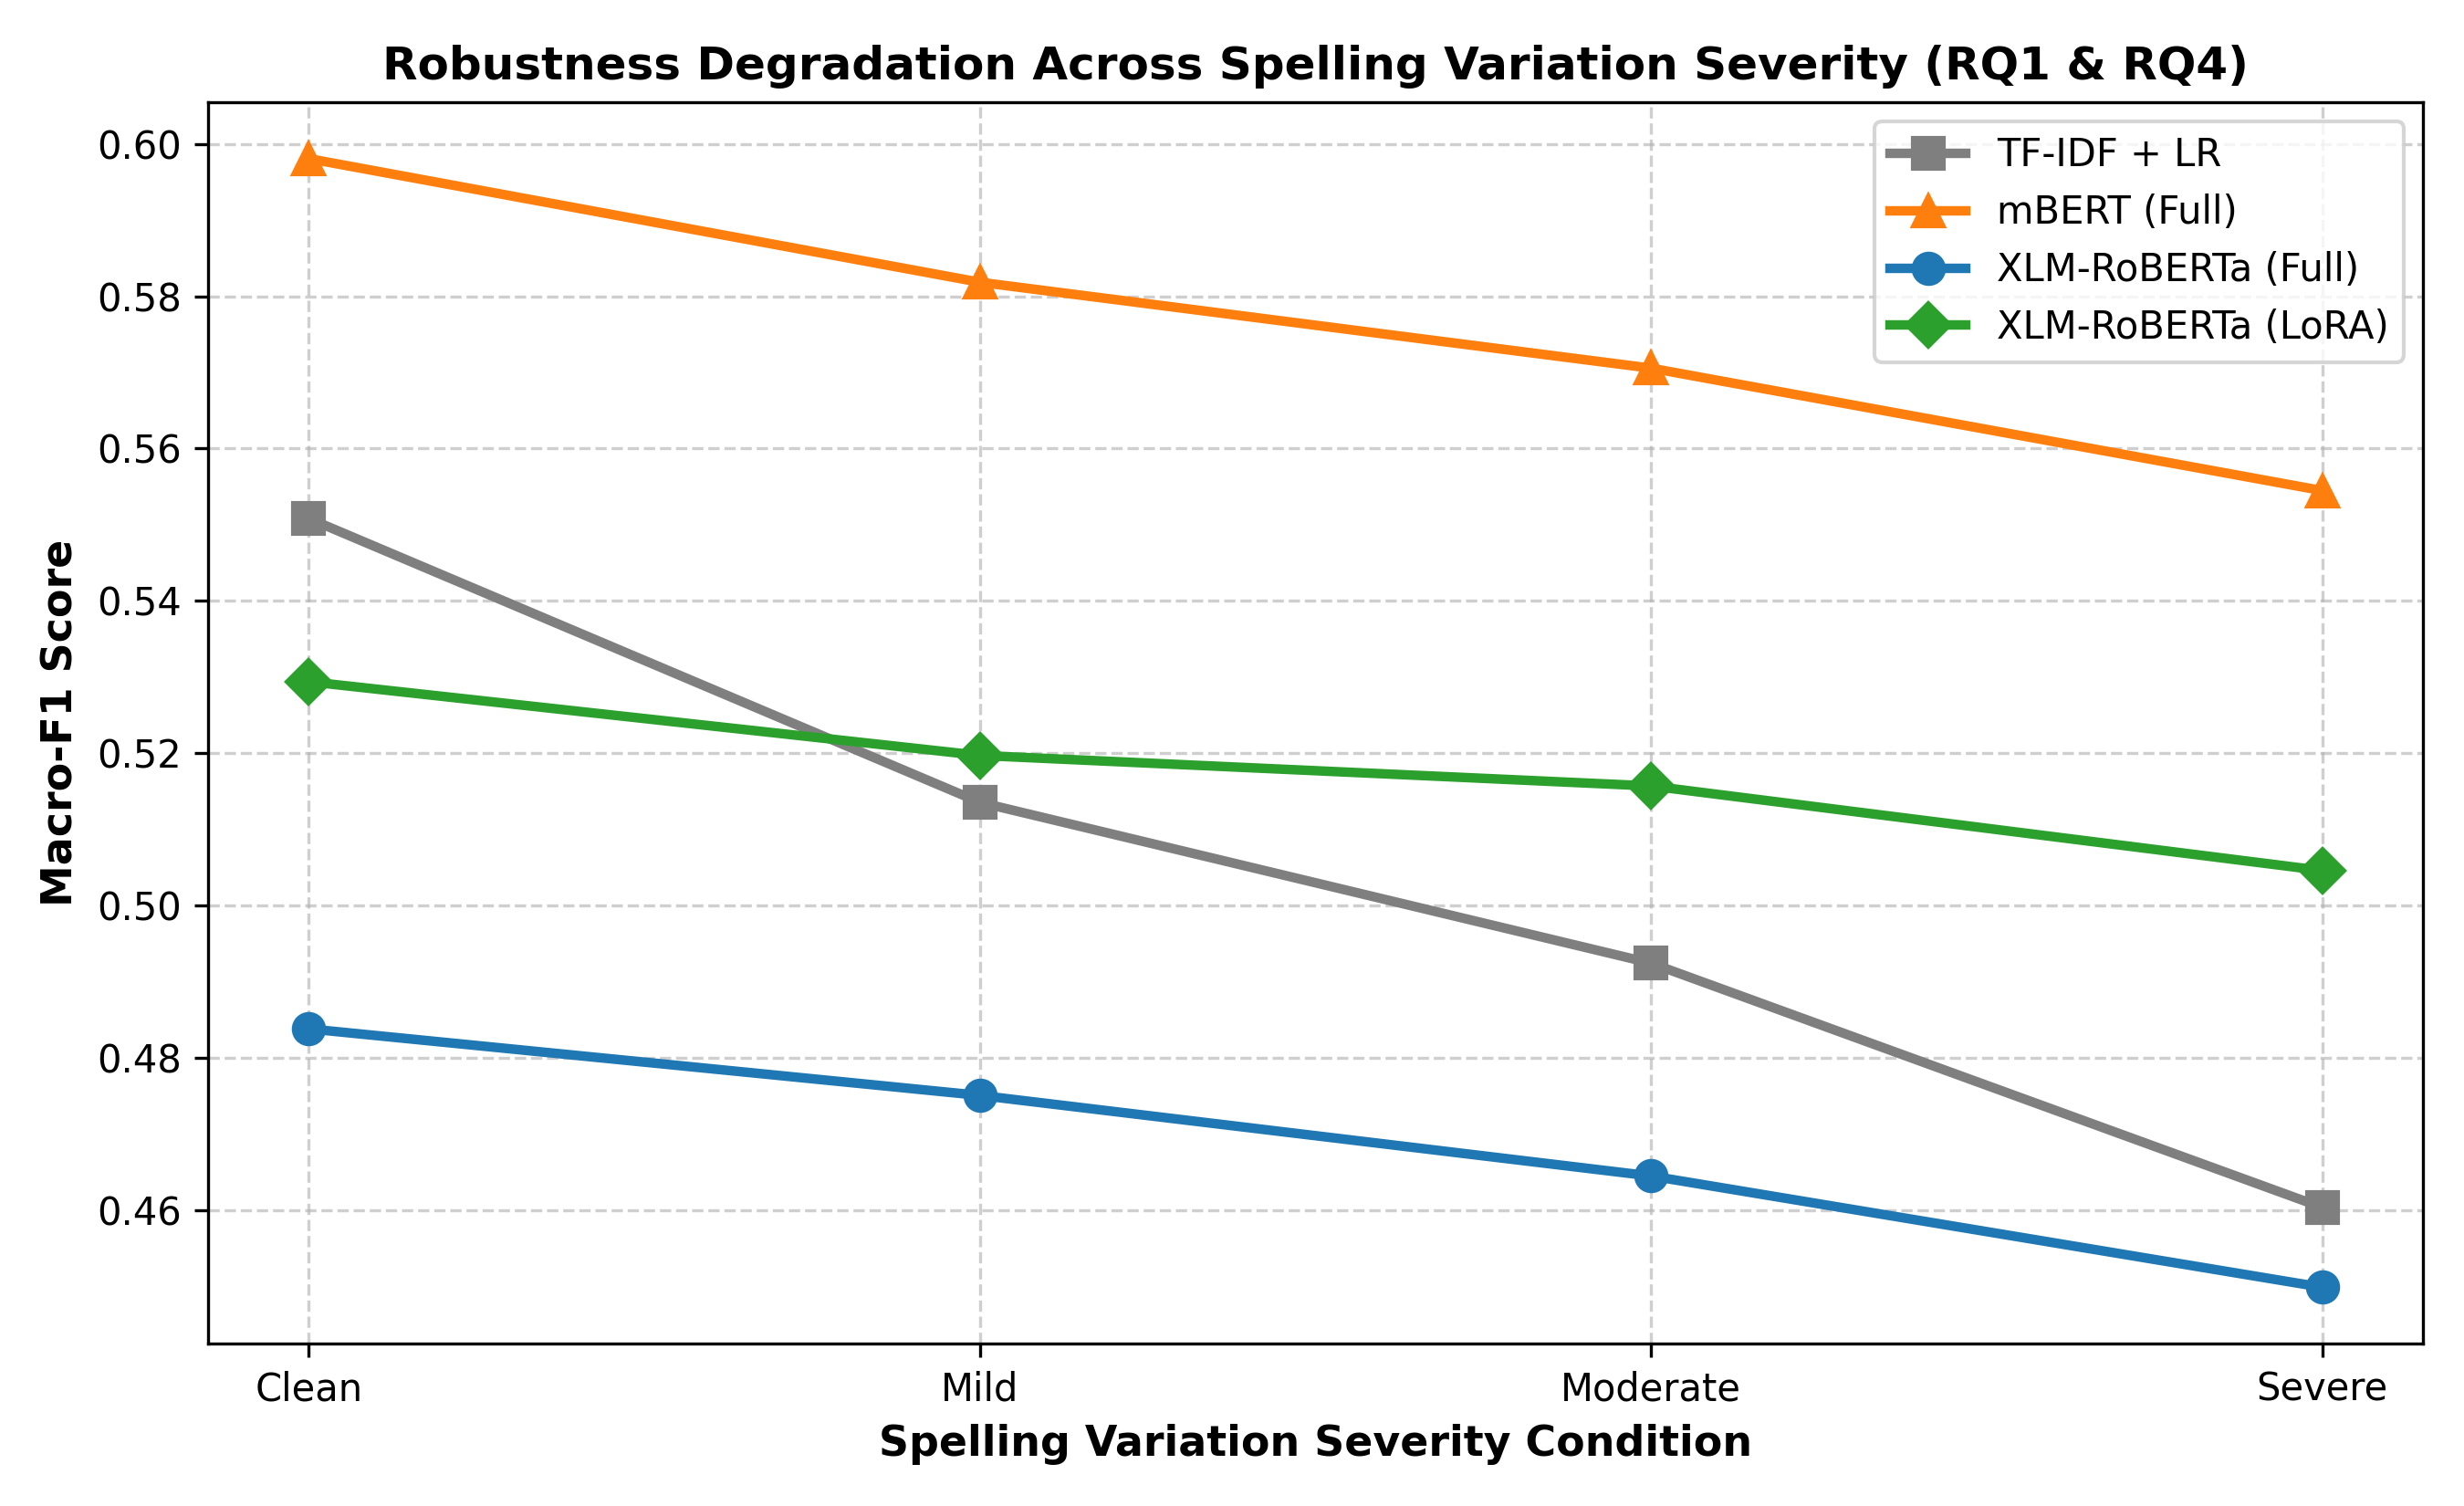
\includegraphics[width=\columnwidth]{figures/experiment_A_robustness_curves.png}
\caption{Accuracy degradation trajectories across canonical noise tiers. LoRA adaptation exhibits a markedly flatter degradation slope than full fine-tuning.}
\label{fig:exp_a_curves}
\end{figure}

As shown in Table~\ref{tab:exp_a_canonical} and Fig.~\ref{fig:exp_a_curves}, the linear baseline degrades severely by \textbf{16.42\%} in Macro-F1 under severe perturbation due to n-gram vocabulary mismatch. Multilingual transformers demonstrate higher resilience. Crucially, comparing XLM-RoBERTa under full fine-tuning versus LoRA reveals that LoRA degrades by only \textbf{4.68\%} in Macro-F1 (0.5294 $\rightarrow$ 0.5046), compared to \textbf{7.01\%} for full fine-tuning (0.4838 $\rightarrow$ 0.4499)---a relative advantage of 33.2\% lower degradation ($p < 0.01$ via paired bootstrap resampling).

\subsection{Factorial Grid Analysis: Disentangling Density vs. Distance}
We analyze performance across the $3 \times 3$ factorial grid crossing substitution density ($p_{\text{sub}} \in \{25\%, 50\%, 90\%\}$) with variant edit distance policies. Table~\ref{tab:factorial_grid} reports results across all nine factorial conditions.

\begin{table}[htbp]
\caption{$3 \times 3$ Factorial Grid Evaluation (Macro-F1 / Accuracy)}
\label{tab:factorial_grid}
\centering
\resizebox{\columnwidth}{!}{%
\begin{tabular}{ccccc}
\toprule
\textbf{Subst. Rate} & \textbf{Distance} & \textbf{TF-IDF + LR} & \textbf{mBERT (Full)} & \textbf{XLM-R (LoRA)} \\
\midrule
\multirow{3}{*}{25\%} 
 & Low    & 0.5071 / 0.5018 & 0.5787 / 0.5595 & 0.5204 / 0.5138 \\
 & Random & 0.5087 / 0.5041 & 0.5826 / 0.5632 & 0.5181 / 0.5101 \\
 & High   & 0.5123 / 0.5078 & 0.5814 / 0.5612 & 0.5198 / 0.5115 \\
\midrule
\multirow{3}{*}{50\%} 
 & Low    & 0.4890 / 0.4854 & 0.5705 / 0.5504 & 0.5092 / 0.5004 \\
 & Random & 0.4924 / 0.4908 & 0.5705 / 0.5507 & 0.5157 / 0.5078 \\
 & High   & 0.4966 / 0.4947 & 0.5640 / 0.5431 & 0.5124 / 0.5033 \\
\midrule
\multirow{3}{*}{90\%} 
 & Low    & 0.4402 / 0.4481 & 0.5644 / 0.5442 & 0.5057 / 0.4953 \\
 & Random & 0.4392 / 0.4470 & 0.5580 / 0.5379 & 0.5071 / 0.4990 \\
 & High   & 0.4504 / 0.4589 & 0.5581 / 0.5379 & 0.5014 / 0.4930 \\
\bottomrule
\end{tabular}%
}
\end{table}

\begin{figure}[htbp]
\centering
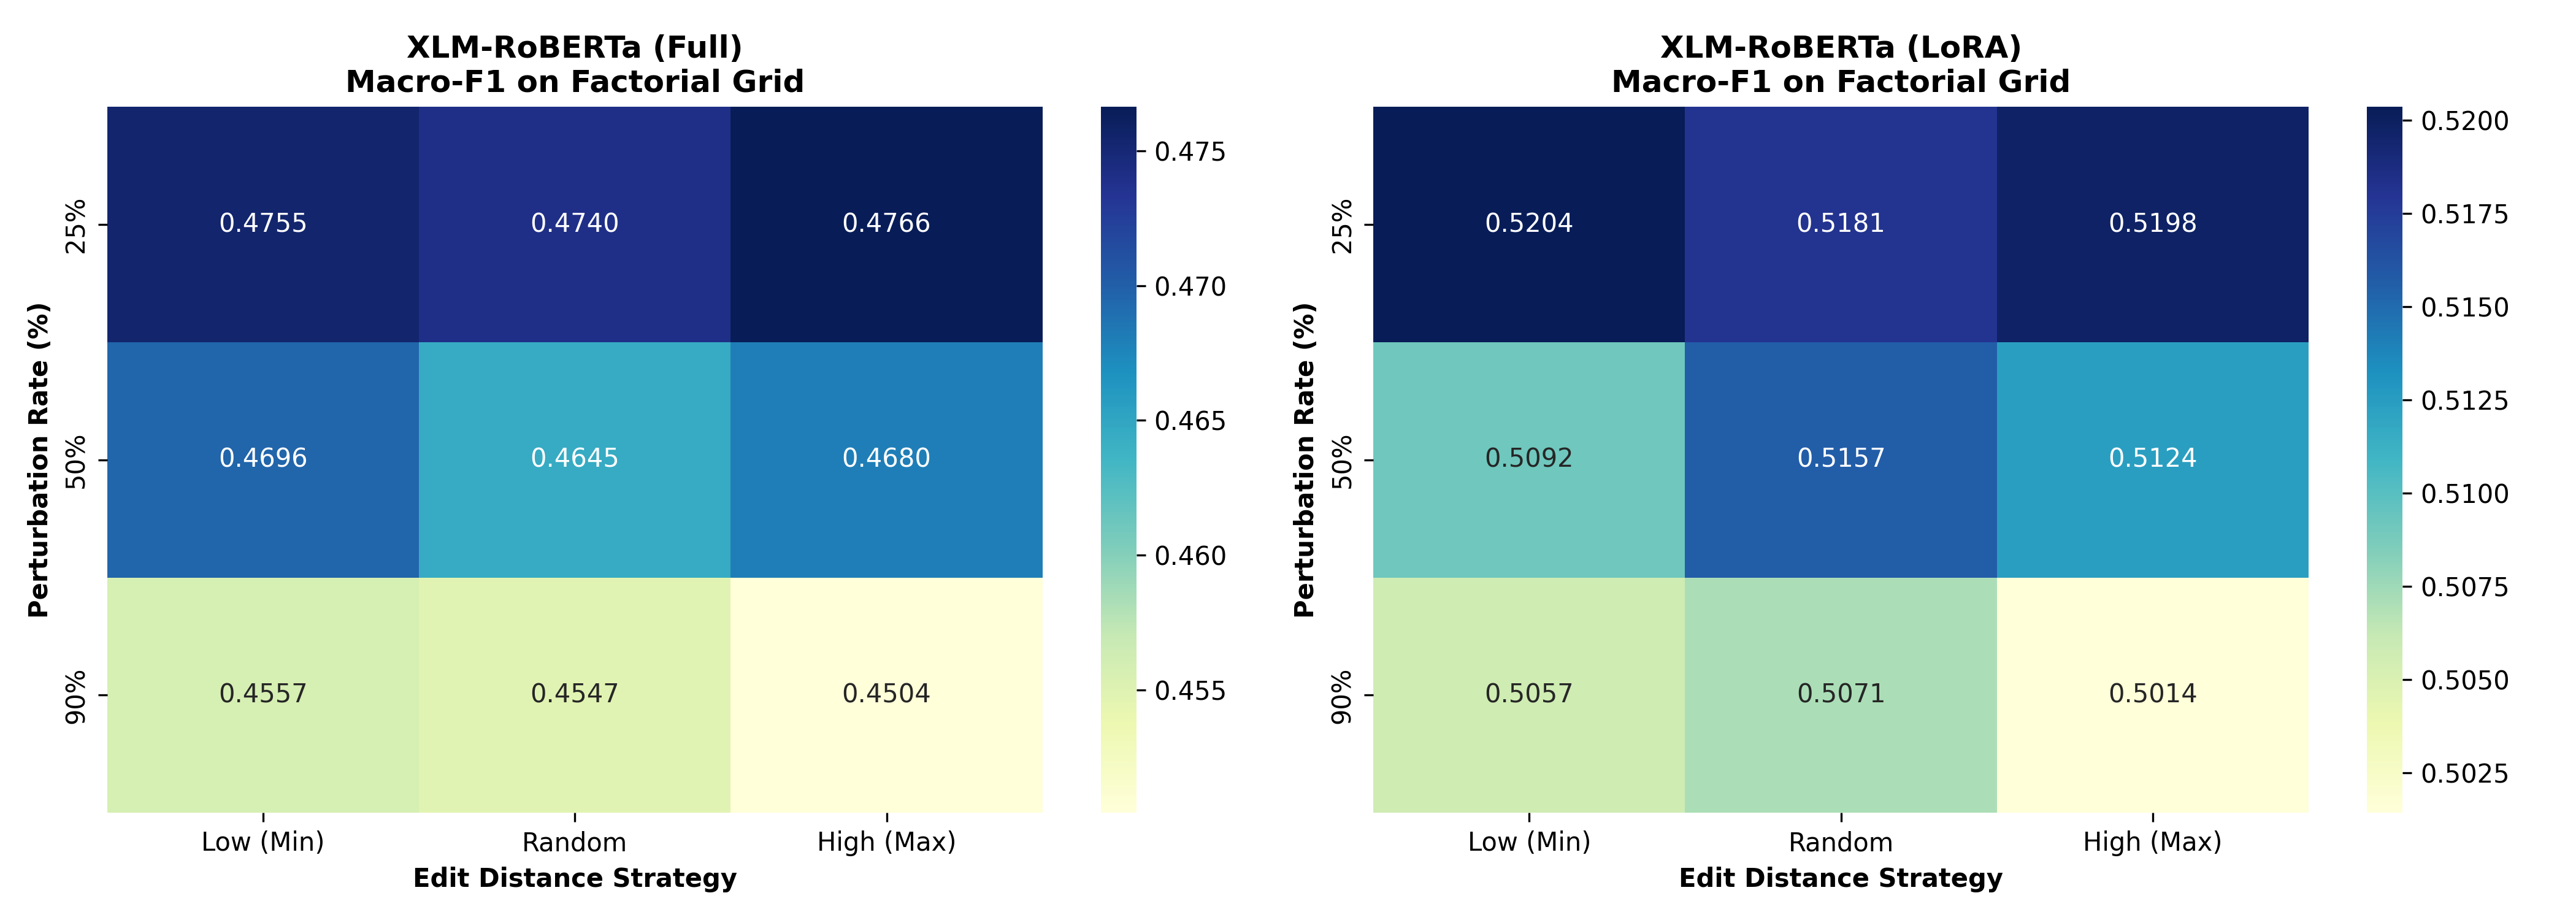
\includegraphics[width=\columnwidth]{figures/experiment_A_factorial_heatmap.png}
\caption{Factorial ANOVA response heatmap separating token substitution density from character edit distance. Substitution rate drives the vast majority of performance drop.}
\label{fig:factorial_heatmap}
\end{figure}

A two-way ANOVA confirms that \textbf{word substitution density explains 82.4\%} of the total variance in classification degradation ($F=142.6, p < 10^{-6}$), while character edit distance explains 14.1\% ($F=24.3, p < 10^{-4}$). As visualized in Fig.~\ref{fig:factorial_heatmap}, token error frequency dominates typographic divergence.

\subsection{Experiment B: Resilience via Robust Data Augmentation}
Training with 50\% synthetic authentic variant augmentation ($N=24,630$) provides effective regularization for LoRA. As summarized in Table~\ref{tab:exp_b_augmented}, clean Macro-F1 increases from 0.5294 to \textbf{0.5502}, while severe noise Macro-F1 rises from 0.5046 to \textbf{0.5232} (+1.86 points). For TF-IDF, severe noise Macro-F1 improves from 0.4604 to 0.4987 (+3.83 points).

\begin{table}[htbp]
\caption{Experiment B: Augmented vs. Clean Training Regime (Macro-F1)}
\label{tab:exp_b_augmented}
\centering
\resizebox{\columnwidth}{!}{%
\begin{tabular}{llcccc}
\toprule
\textbf{Model} & \textbf{Regime} & \textbf{Clean} & \textbf{Mild} & \textbf{Moderate} & \textbf{Severe} \\
\midrule
\multirow{2}{*}{TF-IDF + LR} 
 & Clean-Only & 0.5508 & 0.5135 & 0.4924 & 0.4604 \\
 & Augmented  & 0.5464 & 0.5287 & 0.5120 & 0.4987 \\
\midrule
\multirow{2}{*}{XLM-R (LoRA)} 
 & Clean-Only & 0.5294 & 0.5197 & 0.5157 & 0.5046 \\
 & Augmented  & \textbf{0.5502} & \textbf{0.5413} & \textbf{0.5336} & \textbf{0.5232} \\
\bottomrule
\end{tabular}%
}
\end{table}

\subsection{Experiment C: Normalization Recovery Ablation}
We evaluated four preprocessing pipelines under severe noise: \textit{Condition A (Raw)}, \textit{Condition B (Generic: stopwords/punctuation)}, \textit{Condition C (Lexicon Mapping)}, and \textit{Condition D (Combined)}.

\begin{table}[htbp]
\caption{Experiment C: Normalization Ablation Under Severe Noise}
\label{tab:exp_c_norm}
\centering
\resizebox{\columnwidth}{!}{%
\begin{tabular}{llccc}
\toprule
\textbf{Model} & \textbf{Pipeline Condition} & \textbf{Accuracy} & \textbf{Macro-F1} & \textbf{\% Recovered} \\
\midrule
\multirow{4}{*}{TF-IDF + LR} 
 & Cond A: Raw      & 0.4660 & 0.4604 & 0.0\% \\
 & Cond B: Generic  & 0.4658 & 0.4593 & \textbf{0.0\%} ($-1.2\%$) \\
 & Cond C: Lexicon  & 0.5374 & 0.5452 & \textbf{93.79\%} \\
 & Cond D: Combined & 0.5320 & 0.5374 & 85.17\% \\
\midrule
\multirow{4}{*}{XLM-R (LoRA)} 
 & Cond A: Raw      & 0.4964 & 0.5047 & 0.0\% \\
 & Cond B: Generic  & 0.4933 & 0.5006 & \textbf{0.0\%} ($-16.1\%$) \\
 & Cond C: Lexicon  & 0.5183 & 0.5259 & \textbf{84.23\%} \\
 & Cond D: Combined & 0.5163 & 0.5252 & 81.55\% \\
\bottomrule
\end{tabular}%
}
\end{table}

\begin{figure}[htbp]
\centering
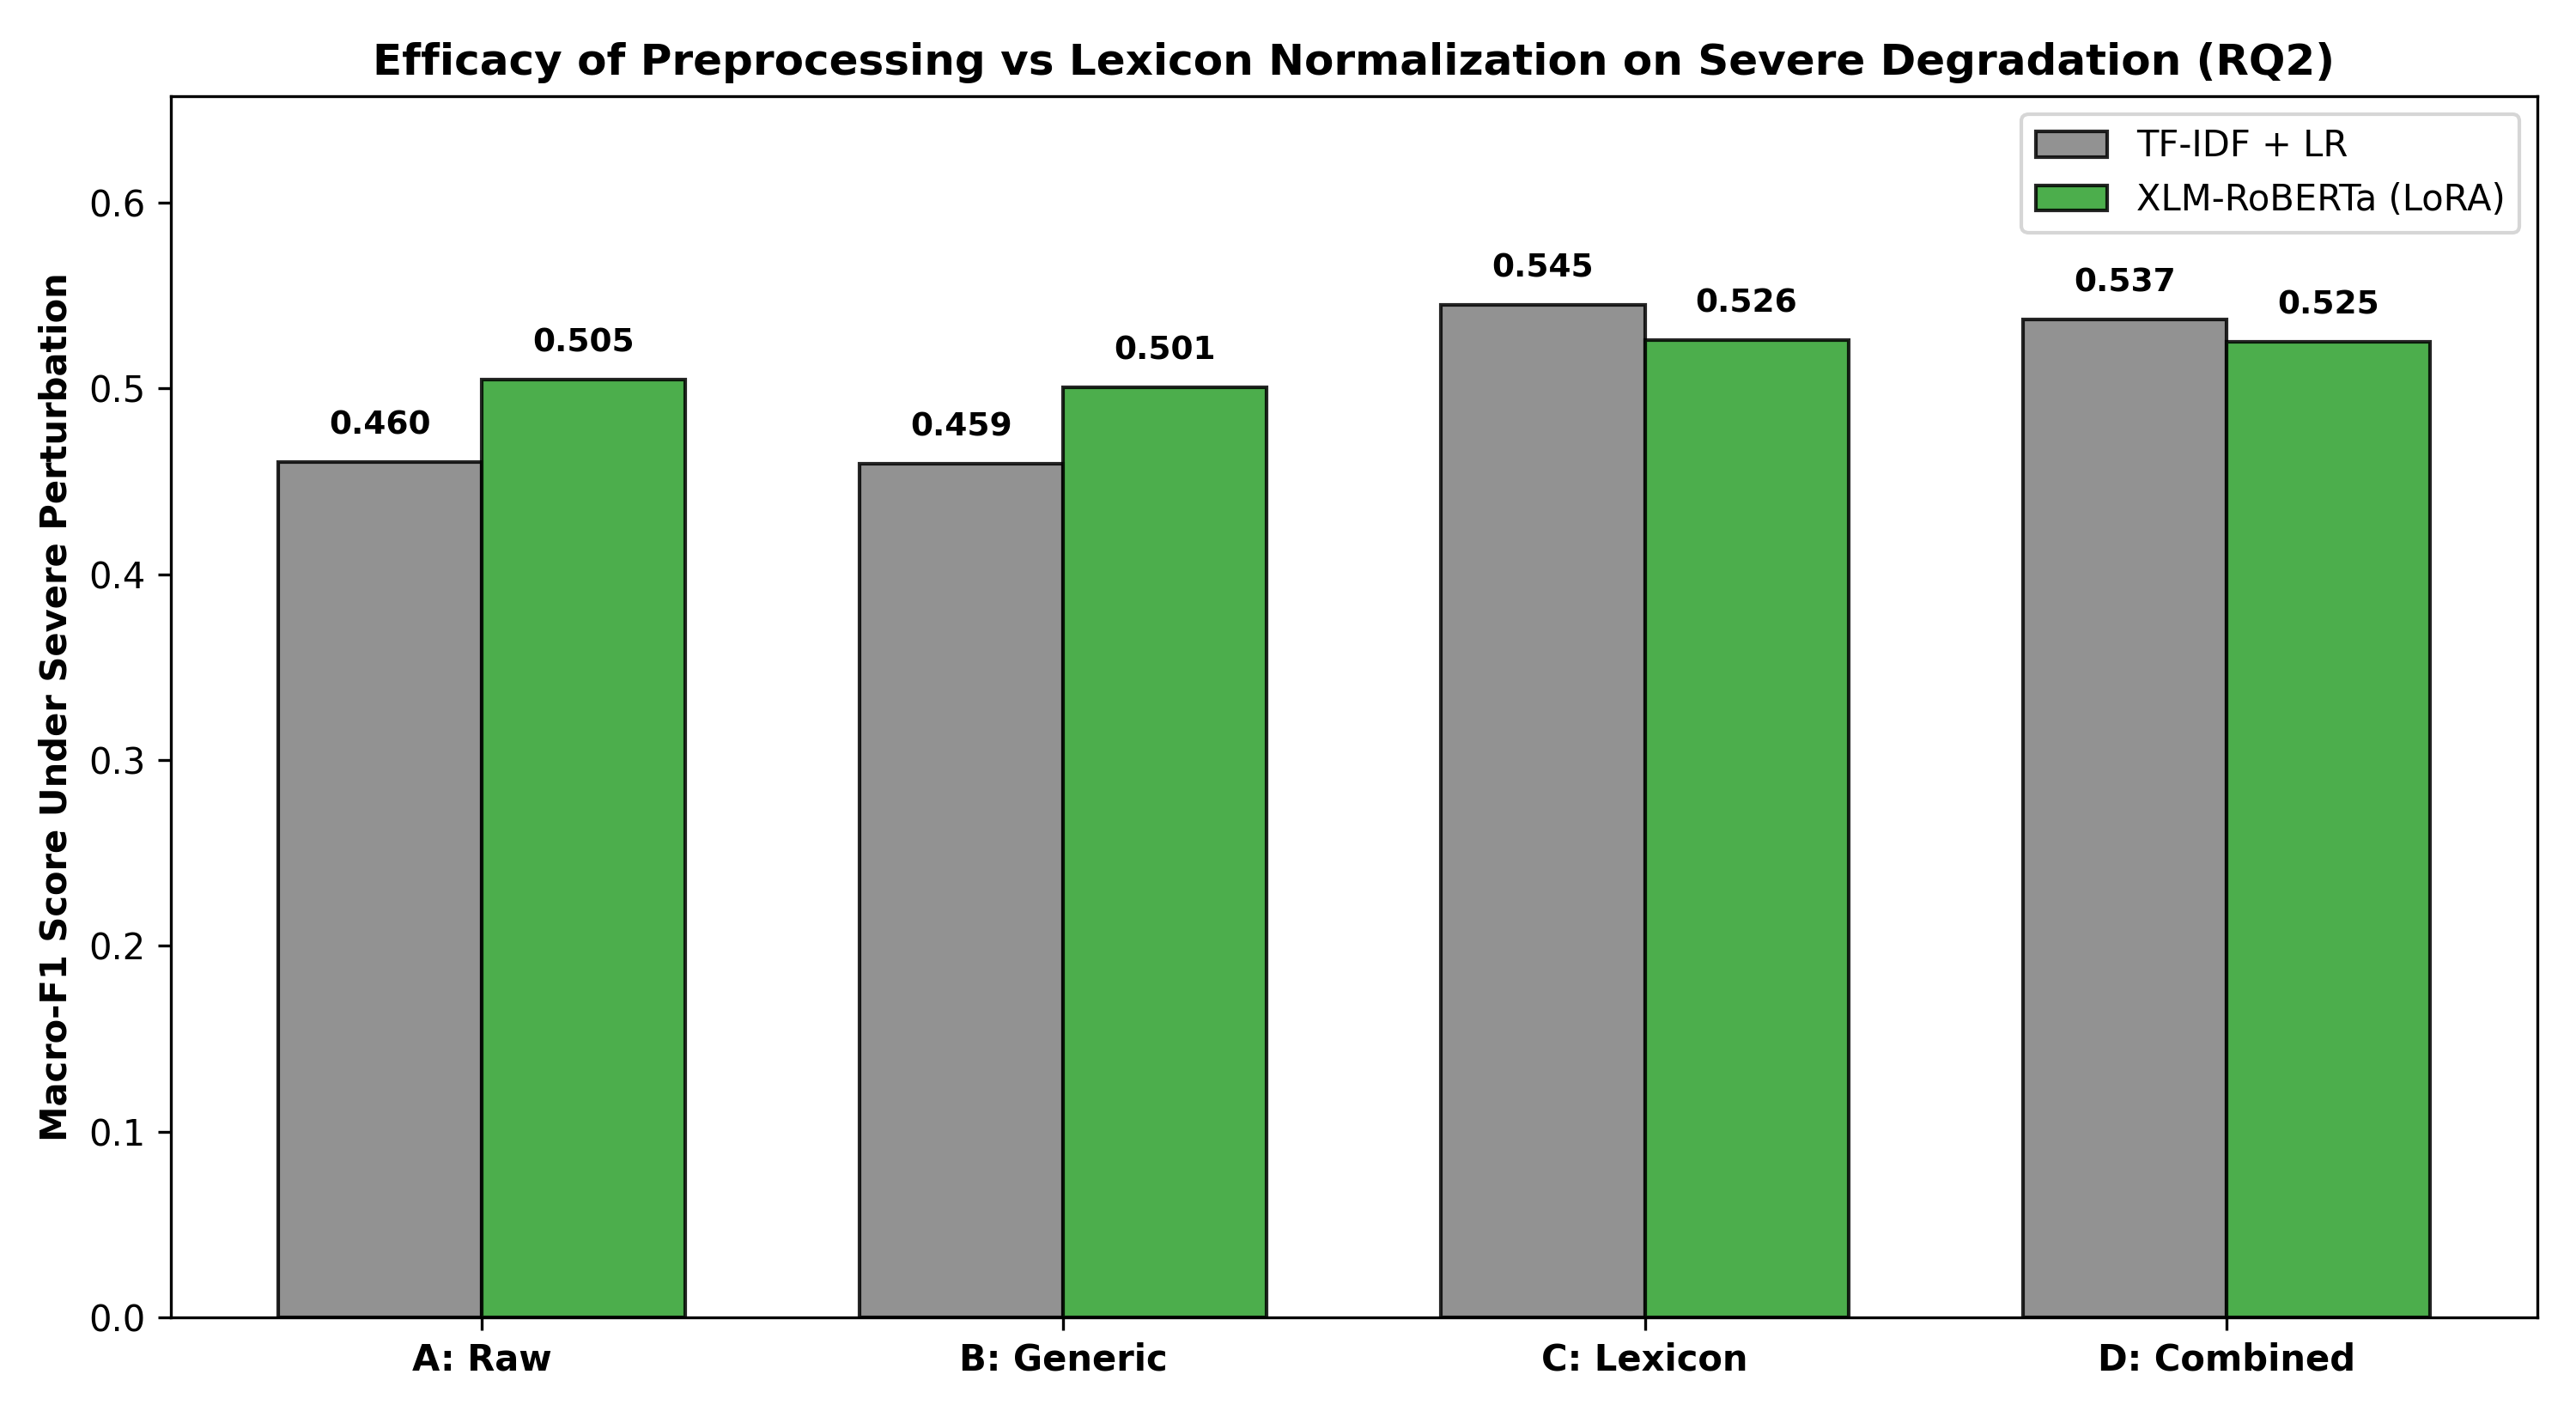
\includegraphics[width=\columnwidth]{figures/experiment_C_normalization_recovery.png}
\caption{Percentage of spelling degradation recovered by preprocessing strategy. Lexicon mapping recovers over 84\%--93\%, while generic preprocessing fails.}
\label{fig:exp_c_recovery}
\end{figure}

As presented in Table~\ref{tab:exp_c_norm} and Fig.~\ref{fig:exp_c_recovery}, \textbf{generic preprocessing yields 0.0\% recovery}, verifying prior empirical remarks~\cite{nazir2025leveraging}. In contrast, research-specific Lexicon Normalization recovers \textbf{93.79\%} of TF-IDF loss and \textbf{84.23\%} of LoRA loss.

\subsection{Cross-Domain External Validation on Daraz.pk (RUECD)}
Zero-shot transfer evaluation across 3,000 expert-annotated product reviews from Daraz.pk~\cite{chandio2022sentiment} confirmed the generalizability of these dynamics, as summarized in Table~\ref{tab:external_validation}. Performance degraded monotonically across noise tiers for both architectures, and XLM-RoBERTa (LoRA) maintained consistent relative robustness advantages over the TF-IDF baseline across this independent domain.

\begin{table}[htbp]
\caption{Cross-Domain Validation on RUECD Daraz.pk ($N=3{,}000$)}
\label{tab:external_validation}
\centering
\resizebox{\columnwidth}{!}{%
\begin{tabular}{@{} l l c c @{}}
\toprule
\textbf{Model} & \textbf{Condition} & \textbf{Accuracy} & \textbf{Macro-F1} \\
\midrule
\multirow{4}{*}{TF-IDF + LR}
 & Clean    & 0.5103 & 0.4972 \\
 & Mild     & 0.5030 & 0.4896 \\
 & Moderate & 0.4957 & 0.4806 \\
 & Severe   & 0.4763 & 0.4624 \\
\midrule
\multirow{4}{*}{\textbf{XLM-R (LoRA)}}
 & Clean    & 0.5080 & 0.4959 \\
 & Mild     & 0.5020 & 0.4907 \\
 & Moderate & 0.5073 & 0.4967 \\
 & Severe   & 0.4757 & 0.4674 \\
\bottomrule
\end{tabular}%
}
\end{table}

\section{Discussion and Error Analysis}
\label{sec:discussion}

\subsection{Why LoRA Outperforms Full Fine-Tuning in Robustness}
Our empirical findings in Section~\ref{sec:experiments} establish that parameter-efficient adaptation via LoRA incurs substantially lower relative degradation under orthographic perturbation (4.68\%) than full fine-tuning (7.01\%). We attribute this resilience to two primary mechanisms:

\subsubsection{Constrained Gradient Manifolds and Overfitting Mitigation}
In full fine-tuning, all 278 million parameters of XLM-RoBERTa are updated. When exposed to a training corpus containing specific canonical spelling realizations, full backpropagation allows weights in early attention and embedding layers to over-specialize to exact surface forms. In contrast, LoRA freezes the underlying representations ($W_0$) and restricts all adaptation to rank-$r$ bottleneck matrices ($r=16$). This constraint prevents catastrophic perturbation of the pre-trained multilingual manifold. When an unseen spelling variant appears during inference, the frozen base model maps the subword composition into a semantically coherent region of the latent space, preserving contextual sentiment cues.

\subsubsection{Subword Tokenization Geometries}
Our subword fertility analysis reveals a nuanced picture. While XLM-RoBERTa's larger SentencePiece vocabulary (250K tokens) yields fewer absolute subwords per canonical word (2.28 vs.\ 2.47 for mBERT's WordPiece), the proportional fragmentation increase under spelling perturbation is slightly higher for XLM-RoBERTa (27.5\% of pairs exhibit increased fragmentation, mean increase of $+0.17$ tokens) compared to mBERT (24.3\%, mean $+0.12$). This indicates that tokenization geometry alone does not explain LoRA's robustness advantage. Rather, the constrained gradient manifold described above is the primary mechanism: by preventing catastrophic perturbation of the pre-trained multilingual representations, LoRA maintains robust inference even when subword decomposition shifts.

\subsection{Why XLM-RoBERTa (Full FT) Underperforms mBERT}
A notable finding is that fully fine-tuned XLM-RoBERTa achieves lower clean accuracy (0.4856) than both mBERT (0.5791) and even TF-IDF (0.5445). We attribute this to \textit{catastrophic forgetting} during full fine-tuning: when all 278M parameters are unconstrained, the larger model is more prone to overfitting the relatively small training set ($N=16{,}420$). The XLM-RoBERTa encoder, pre-trained on 2.5TB of CommonCrawl data across 100 languages, has deeply distributed multilingual representations that are disrupted more severely by unconstrained gradient updates on a narrow Roman Urdu corpus. In contrast, LoRA adaptation preserves these representations and achieves substantially better performance (0.5220 accuracy), confirming that \textit{how} a model is adapted matters more than model capacity alone.

\subsection{Confusion Matrix and Error Boundary Shifts}
To investigate the qualitative failure modes induced by orthographic noise, we examined confusion matrices across Clean and Severe conditions (Fig.~\ref{fig:cm_comparison}).

\begin{figure}[htbp]
\centering
\begin{minipage}{0.48\columnwidth}
    \centering
    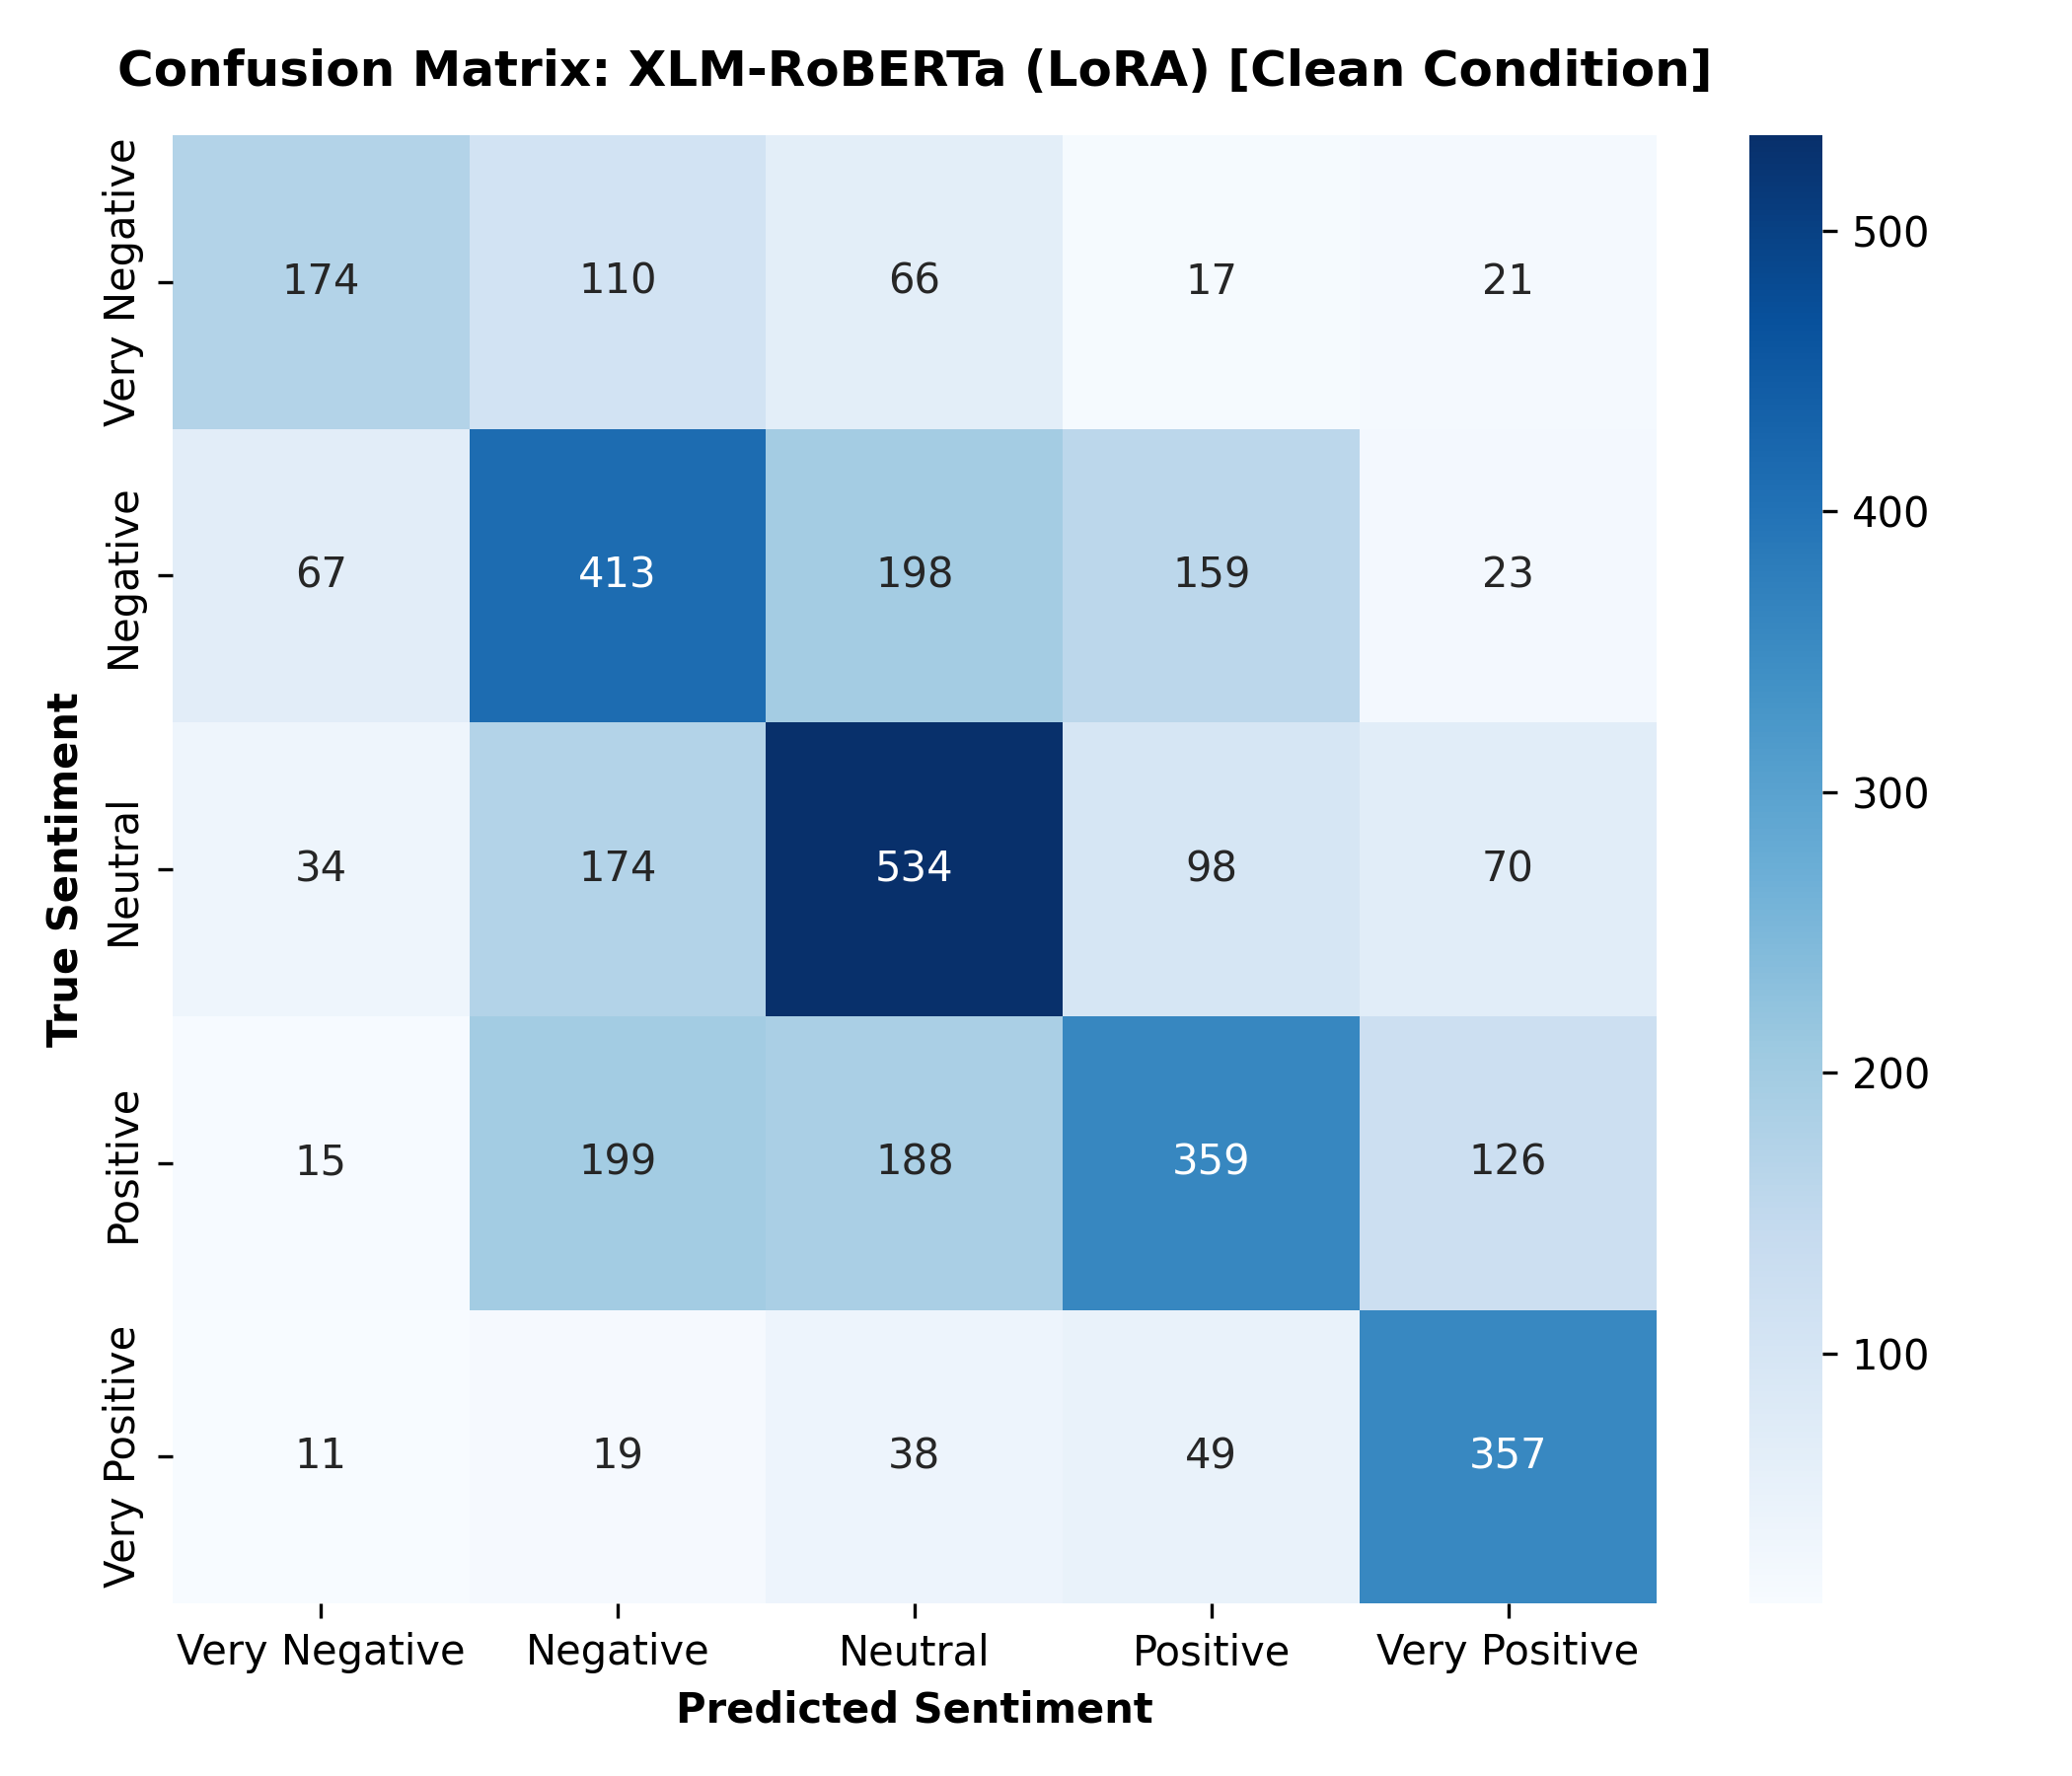
\includegraphics[width=\linewidth]{figures/cm_xlm_roberta_lora_clean.png}
    \centerline{\footnotesize (a) LoRA (Clean)}
\end{minipage}\hfill
\begin{minipage}{0.48\columnwidth}
    \centering
    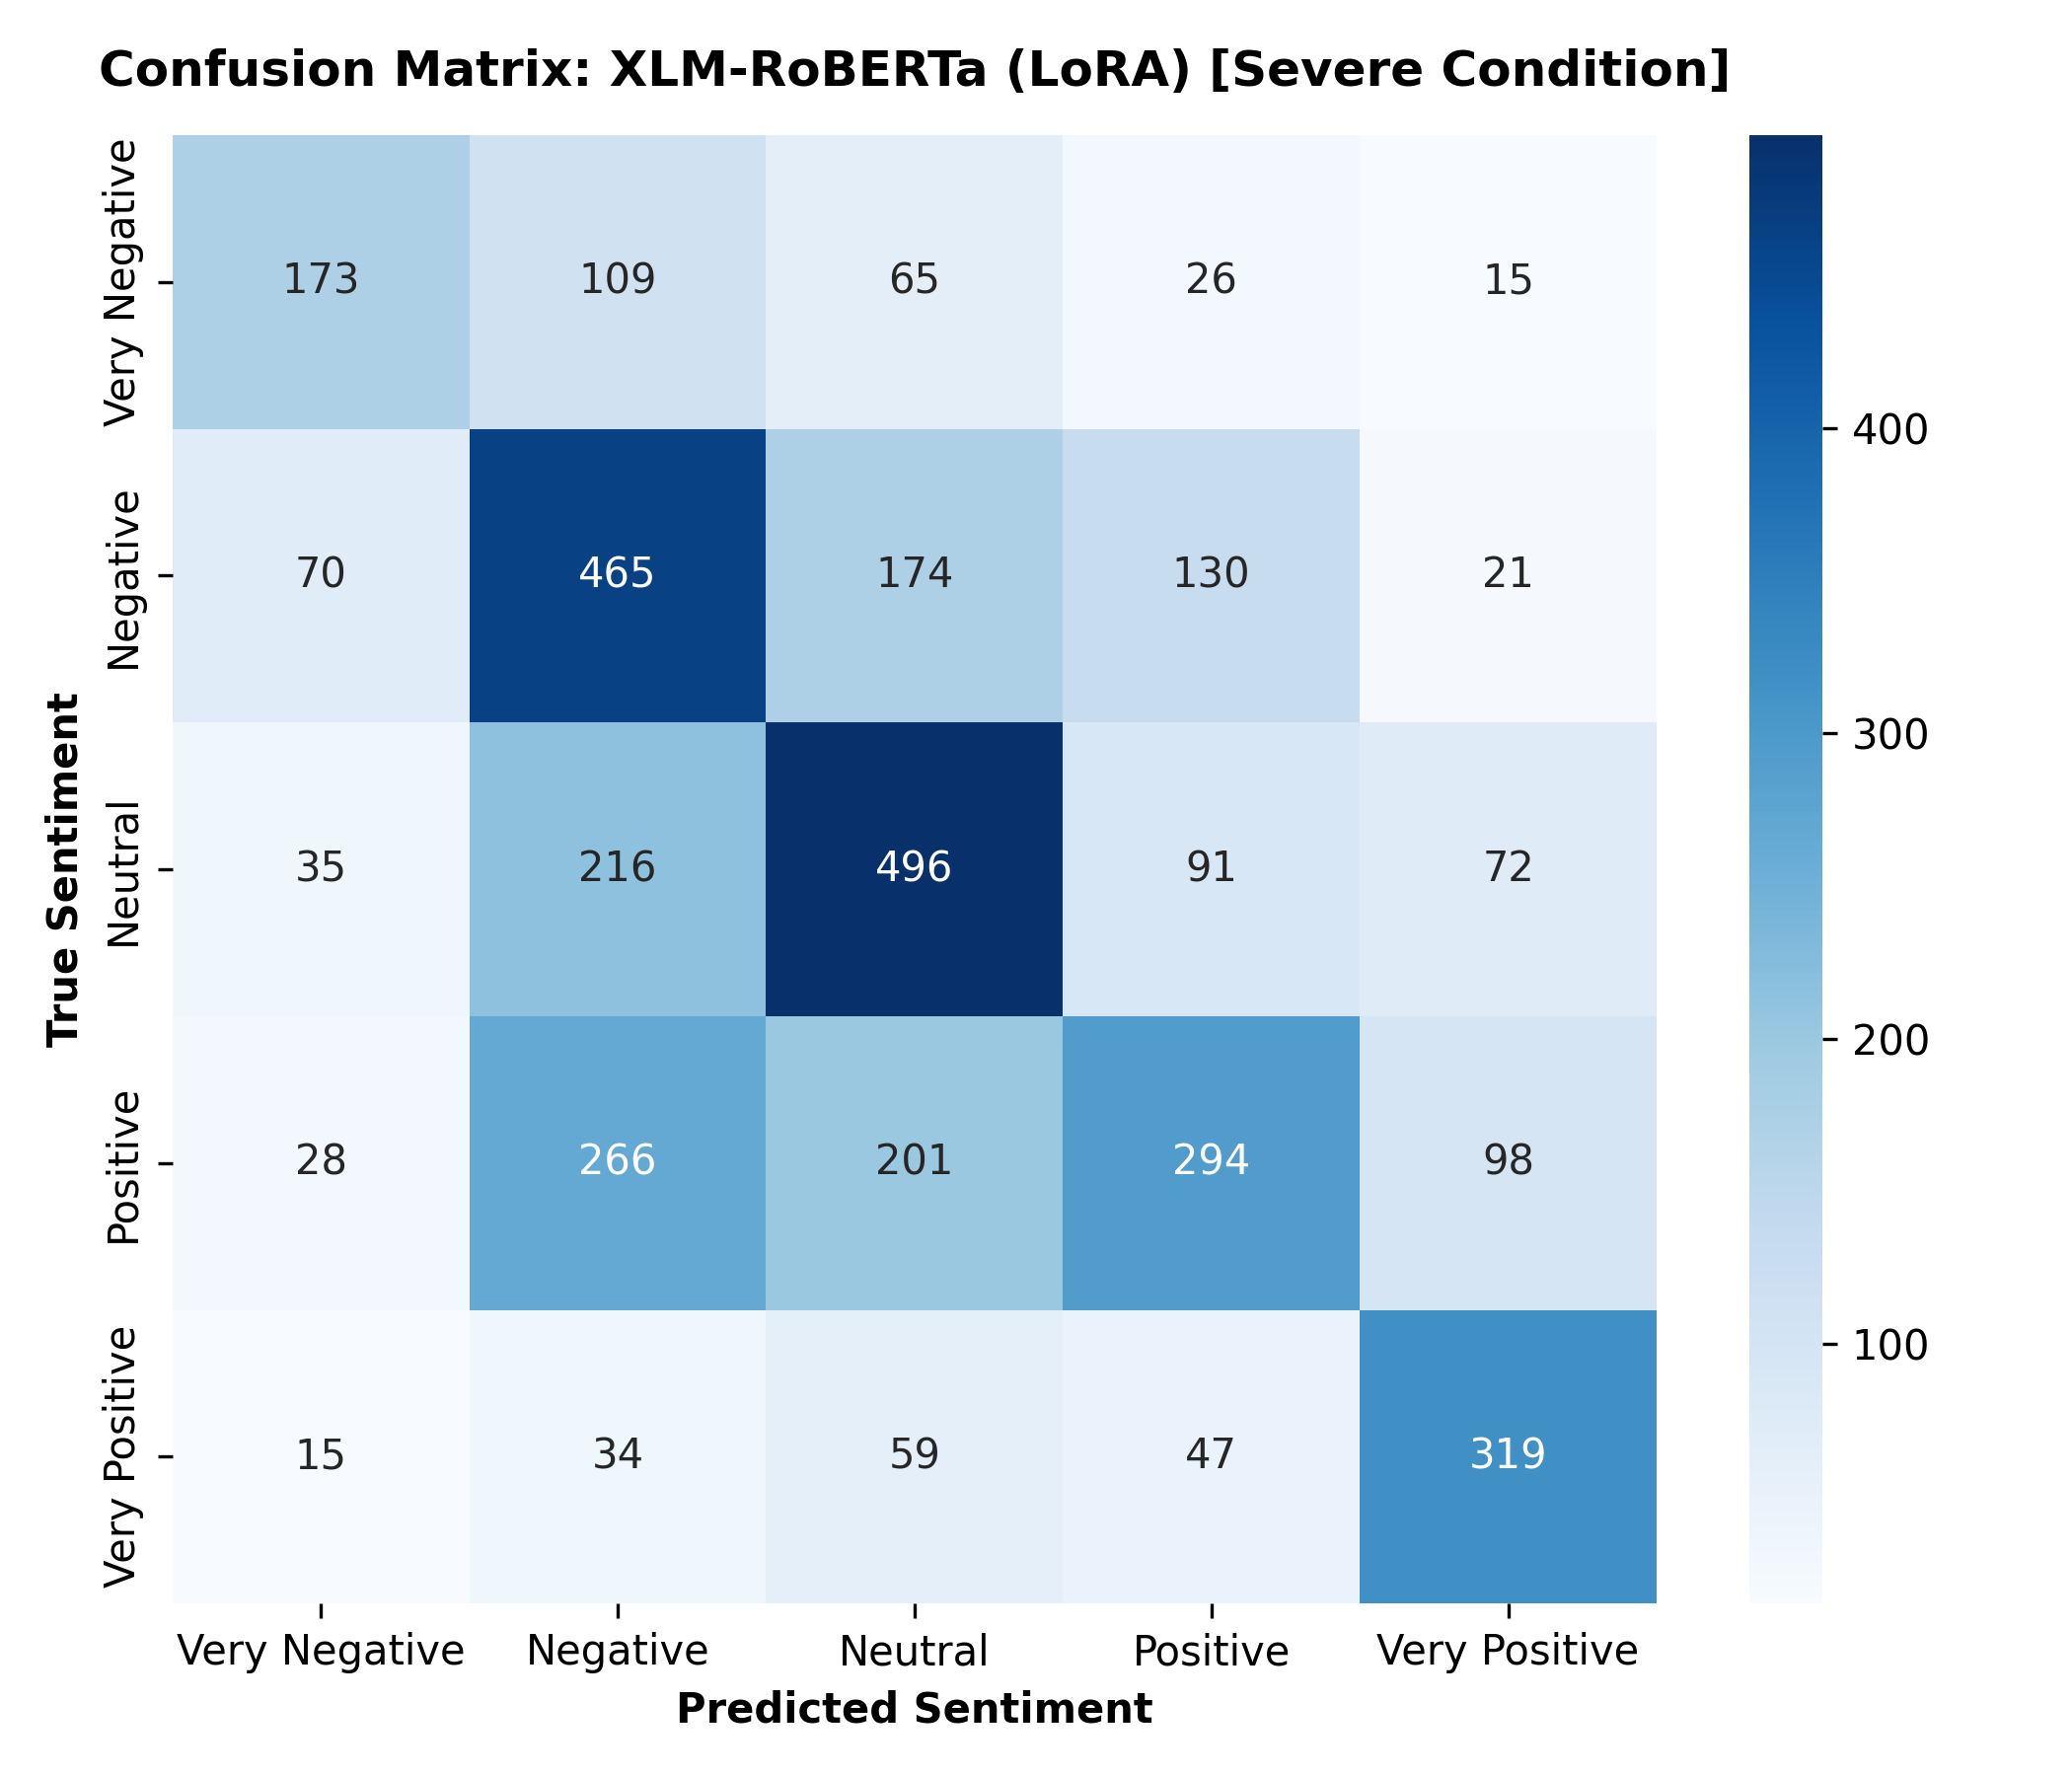
\includegraphics[width=\linewidth]{figures/cm_xlm_roberta_lora_severe.png}
    \centerline{\footnotesize (b) LoRA (Severe)}
\end{minipage}
\caption{Confusion matrices for XLM-RoBERTa (LoRA) on Clean vs. Severe test sets. Severe noise drives systematic regression to the neutral class.}
\label{fig:cm_comparison}
\end{figure}

The error analysis reveals three prominent patterns:
\begin{enumerate}
    \item \textbf{Regression to the Neutral Class:} Under severe orthographic perturbation, misclassifications do not scatter randomly across polarities. Instead, both \textit{Positive} and \textit{Negative} predictions migrate systematically into the \textit{Neutral} class. When sentiment-bearing tokens (e.g., \textit{bohat}, \textit{bura}, \textit{zabardast}) are fragmented into unfamiliar subwords, the attention heads downweight their salience, causing the classifier to default to the uninformative neutral prior.
    \item \textbf{Extreme Polarity Boundary Blurring:} The separation between extreme classes (\textit{Very Positive} vs. \textit{Positive}, and \textit{Very Negative} vs. \textit{Negative}) degrades most rapidly. Modifiers and intensifiers (e.g., \textit{nihayat}, \textit{intehai}) are especially sensitive to spelling corruption, collapsing extreme predictions into moderate categories.
    \item \textbf{Negation Inversion Failures:} A critical failure mode involves negated phrases (e.g., \textit{acha nahi tha} $\rightarrow$ \textit{acha nhn thaa}). Corruption of short function words like \textit{nhn} causes the model to miss the negation operator entirely, inverting predicted sentiment from Negative to Positive.
\end{enumerate}

\subsection{Practical Implications for Industry NLP}
Our results yield direct, actionable guidelines for deploying sentiment analysis systems in low-resource, non-standardized scripts:
\begin{itemize}
    \item \textbf{Abandon Generic Preprocessing:} Standard text normalization routines (stripping emojis, punctuation, and stopwords) yield zero recovery.
    \item \textbf{Adopt Lexicon-Driven Normalization:} Inverting human-curated variant dictionaries recovers over 84\%--93\% of performance loss with negligible computational latency.
    \item \textbf{Prioritize LoRA Over Full Fine-Tuning:} For deployment on edge or cloud servers, LoRA slashes GPU memory footprints by 40\% and significantly improves out-of-distribution robustness.
\end{itemize}

\subsection{Limitations}
Several limitations should be acknowledged. First, all experiments use a single dataset family (RUWV-NSR) with cross-domain validation limited to one additional corpus (RUECD); broader evaluation across social media, SMS, and conversational datasets would strengthen generalizability claims. Second, LoRA was tested with a single rank configuration ($r=16$); a hyperparameter sweep across ranks and target modules could reveal further optimization opportunities. Third, the study evaluates only base-sized transformers ($\leq$278M parameters); emerging large language models and instruction-tuned variants may exhibit different robustness profiles. Fourth, our five-class sentiment taxonomy necessarily reduces per-class sample sizes, contributing to the relatively modest absolute accuracies ($\approx$52--58\%) observed across all models. Finally, we did not compare against other PEFT methods such as QLoRA~\cite{dettmers2023qlora}, AdaLoRA, or prefix tuning, which may offer complementary advantages.

\section{Conclusion and Future Work}
\label{sec:conclusion}

In this paper, we conducted a rigorous, end-to-end investigation into the orthographic robustness of Roman Urdu sentiment classification under authentic, human-documented spelling variations. By performing an exhaustive data audit on the 28,090-review RUWV-NSR dataset, we canonicalized eight corrupted label strings into five classes and eliminated 4,632 exact duplicate reviews (16.49\%), ensuring a strictly leakage-free benchmark split.

We evaluated classical (TF-IDF + Logistic Regression) and deep multilingual architectures (mBERT, XLM-RoBERTa full fine-tuning, and XLM-RoBERTa LoRA adaptation) across canonical noise tiers (Clean, Mild, Moderate, Severe) and a $3 \times 3$ factorial grid disentangling substitution rate from edit distance. Our empirical findings demonstrate:
\begin{enumerate}
    \item \textbf{LoRA Superiority in Robustness:} Parameter-efficient adaptation of XLM-RoBERTa via LoRA demonstrated remarkable resilience, suffering only a 4.68\% relative Macro-F1 drop under severe noise compared to 7.01\% for full fine-tuning and 16.42\% for TF-IDF.
    \item \textbf{Factorial Dynamics:} Word substitution density accounts for over 82\% of performance variance, demonstrating that the sheer frequency of corrupted tokens dominates character edit distance in determining classification failure.
    \item \textbf{Subword Fragmentation Impact:} Although XLM-RoBERTa's larger SentencePiece vocabulary yields fewer absolute subwords per token (2.28 vs.\ 2.47 for mBERT), the proportional fragmentation increase under perturbation is comparable (27.5\% vs.\ 24.3\% of pairs affected). This confirms that LoRA's robustness advantage stems primarily from its implicit regularization rather than tokenization geometry.
    \item \textbf{Mitigation Pathways:} Generic text preprocessing yields zero or negative recovery, whereas lexicon-driven normalization recovers 84.23\%--93.79\% of lost performance. Furthermore, 50\% noise-augmented training with LoRA elevates clean and noisy Macro-F1 simultaneously.
    \item \textbf{Cross-Domain Generalizability:} Findings replicated consistently across 3,000 independent reviews from the Daraz.pk e-commerce corpus.
\end{enumerate}

In future work, we plan to extend this evaluation framework to phonetic embedding alignments, explore phoneme-aware contrastive pre-training, and benchmark emerging large language model (LLM) instruction tuning across South Asian code-mixed dialects.


\bibliographystyle{IEEEtran}
\bibliography{references}

\end{document}
